% Chapter 1

\chapter{Introducción general} % Main chapter title

\label{Chapter1} % For referencing the chapter elsewhere, use \ref{Chapter1} 
\label{IntroGeneral}

En este capítulo se realiza una breve introducción a la necesidad que condujo al desarrollo del trabajo. Se presentan a los sistemas embebidos, la inteligencia artificial y el estado del arte de dispositivos similares. Asimismo, se explica el objetivo y los alcances del trabajo.

%----------------------------------------------------------------------------------------

% Define some commands to keep the formatting separated from the content 
\newcommand{\keyword}[1]{\textbf{#1}}
\newcommand{\tabhead}[1]{\textbf{#1}}
\newcommand{\code}[1]{\texttt{#1}}
\newcommand{\file}[1]{\texttt{\bfseries#1}}
\newcommand{\option}[1]{\texttt{\itshape#1}}
\newcommand{\grados}{$^{\circ}$}

%----------------------------------------------------------------------------------------

%\section{Introducción}

%----------------------------------------------------------------------------------------
\section{La inteligencia artificial y los sistemas embebidos en la agricultura}

En las últimas décadas, la cosecha de frutos ha experimentado un notable proceso de transformación, impulsado por la integración de tecnologías como los sistemas embebidos y la inteligencia artificial. Estos sistemas, capaces de realizar tareas específicas en tiempo real, se han vuelto fundamentales en la modernización de este sector.

Por otra parte, una de las actividades clave consiste en estimar, con mayor precisión la producción total, dado que esto condiciona diversos aspectos logísticos que deben ser gestionados adecuadamente durante el proceso de recolección.

Actualmente, el volumen de cosecha se estima al contar los frutos por unidad de superficie en una etapa avanzada de desarrollo. Sin embargo, esta evaluación tardía resulta  próxima al momento de la cosecha y presenta grandes dificultades en plantaciones medianas o grandes.

Es en este contexto, el prototipo desarrollado permite recolectar imágenes de la plantación con el fin de realizar una detección de frutos. De esta forma, se obtiene una estimación que facilita la toma de decisiones operativas y
estratégicas \citep{Mendoza2021}.

%----------------------------------------------------------------------------------------

\section{Estado del arte}

Durante la etapa de investigación del trabajo, se realizó una búsqueda de productos comerciales en el mercado local e internacional. Se identificaron algunos con características similares al prototipo desarrollado. Un dato relevante a resaltar es que todos los productos identificados provienen del mercado internacional. No se identificó ningún producto o empresa que ofrezca este tipo de soluciones en el mercado local hasta el momento. A continuación, se describen los hallazgos.

\subsection{Fruitometry}

La tecnología de estimación digital de cultivos (por su sigla en inglés, DCE) de Fruitometry que se muestra en la figura \ref{fig:Fruitometry}, permite a los productores y administradores de huertos observar el desempeño de su cultivo durante la temporada de cosecha. Esto ayuda a maximizar los rendimientos, reducir los costos de cultivo y proporcionar estimaciones antes de la recolección.

Las unidades de campo, instaladas en cuatriciclos y vehículos todo terreno, contienen una variedad de cámaras y sensores destinados a registrar información sobre la densidad de cultivos y las características del huerto. Para cada escaneo de la plantación, se capturan múltiples imágenes. Luego, estas se procesan en tiempo real mediante el motor de inteligencia artificial con aprendizaje profundo para identificar brotes, flores, frutos y características de interés.

Este conjunto de datos se utiliza para elaborar un mapa de calor de densidad resumido y generar informes destinados a la toma de decisiones estratégicas. Dichos informes permiten identificar áreas que requieren atención específica y optimizar la asignación de mano de obra en función de las necesidades del huerto \citep{WEBSITE:Fruitometry2024}.

\vspace{1cm}
\begin{figure}[htbp]
	\centering
	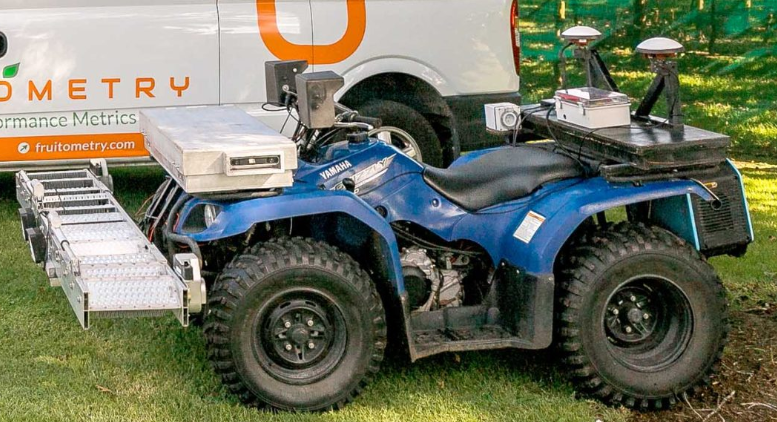
\includegraphics[width=.6\textwidth]{./Figures/Fruitometry.png}
	\caption{Unidad de campo Fruitometry\protect\footnotemark.}
	\label{fig:Fruitometry}
\end{figure}
\vspace{1cm}

\footnotetext{Imagen tomada de \url{https://fruitometry.com/about-fruitometry/.}}

\subsection{Detección de frutos en imágenes de campo}

En un trabajo de investigación realizado en la Universidad Yangling, China, se capturaron imágenes de frutos de kiwis en un huerto bajo diferentes condiciones de iluminación y en distintos momentos del día: mañana, tarde y noche, tanto con flash como sin él. Estas fotografías fueron empleadas para la detección de objetos mediante un modelo llamado Faster R-CNN, implementado con la arquitectura VGG16. Después de aplicar las detecciones, el modelo alcanzó una precisión promedio del 87,61 \%. En la figura \ref{fig:Song2019} se muestran los resultados obtenidos.

Este sistema de visión artificial resultó ser eficaz en la detección de diferentes categorías de frutos en el campo y actuó como un soporte fundamental al robot cosechador. Equipado con este sistema, el robot operó de manera continua durante la temporada de cosecha, lo que representó un avance significativo hacia la automatización de la recolección agrícola \citep{Song2019}.

%\vspace{1cm}

\begin{figure}[htbp]
	\centering
	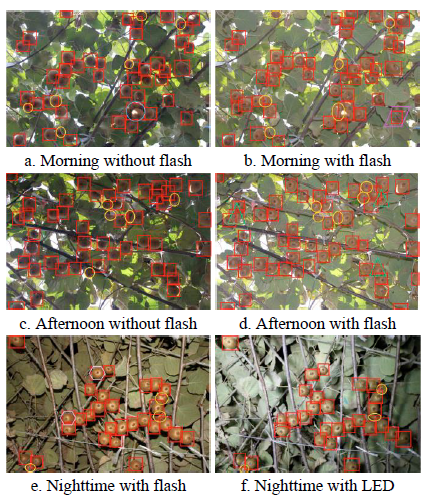
\includegraphics[width=.5\textwidth]{./Figures/Song2019.png}
	\caption{Resultados de una detección de objetos\protect\footnotemark.}
	\label{fig:Song2019}
\end{figure}

%\vspace{1cm}
\footnotetext{Imagen tomada de "Kiwifruit detection in field
images using Faster R-CNN with VGG16".}

\subsection{Calibrado de frutas}

Existen diversos productos comerciales que aplican la detección de objetos para llevar a cabo procesos de clasificación y calibrado de frutas u hortalizas. Estas máquinas que se observan en la figura \ref{fig:calibrado_de_frutas}, estan diseñadas para grandes cadenas de distribución, automatizan la selección y el empaquetado de los productos, lo que incrementa la eficiencia y reduce los tiempos operativos. El sistema funciona a través de una cinta transportadora equipada con cámaras, que capturan imágenes en tiempo real de cada elemento \citep{WEBSITE:Unitec2024}.

%\vspace{1cm}
%\begin{figure}[htbp]
\begin{figure}[h]
	\centering
	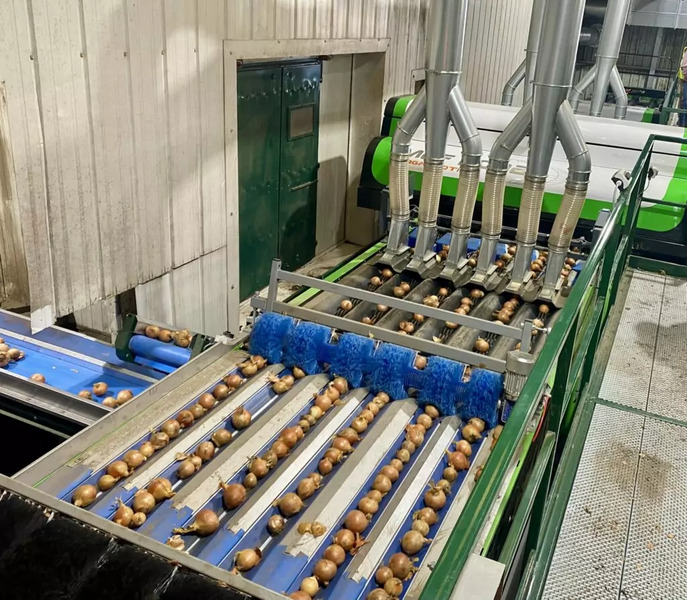
\includegraphics[width=.6\textwidth, height=6cm]{./Figures/calibrado_de_frutas.jpg}
	\caption{Máquina de calibrado de frutas MAF\protect\footnotemark.}
	\label{fig:calibrado_de_frutas}
\end{figure}
%\vspace{1cm}

\footnotetext{Imagen tomada de \url{https://tongengineering.com/product/maf-roda-weight-grading/.}}

Además de identificar cada objeto, las cámaras registran una serie de parámetros importantes, como el diámetro, la longitud, la forma y, en algunos casos, el color. Estos datos se procesan con algoritmos de visión artificial, que clasifican los productos según criterios preestablecidos de calidad.

\subsection{Estimación de cosechas mediante imágenes satelitales y drones}

La teledetección se consolidó como una herramienta clave para la estimación de cosechas y el monitoreo de cultivos a gran escala. En la figura \ref{fig:drones_en_cultivos} se observa que la combinación de imágenes satelitales de alta resolución, sensores multiespectrales y drones con cámaras especializadas posibilita la generación de modelos predictivos del rendimiento agrícola. Estos sistemas proporcionan información temprana sobre el estado vegetativo de los cultivos, lo que facilita la toma de decisiones en diferentes etapas de la producción.

Diversos estudios demostraron que la integración de índices de vegetación, como el NDVI (por su sigla en inglés, \textit{Normalized Difference Vegetation Index}), junto con técnicas de aprendizaje automático, ofrecen resultados consistentes en la predicción del volumen de cosecha en plantaciones frutales y agrícolas. A diferencia de los métodos manuales de conteo de frutos, estas tecnologías permiten la evaluación periódica y no invasiva de grandes extensiones de terreno, lo que contribuye a la reducción de costos operativos y a una mayor precisión en la planificación logística.

Por otro lado, la ventaja de estas soluciones radica en su capacidad de escalar desde parcelas individuales hasta áreas regionales, lo que las convierte en una herramienta estratégica para el análisis de la producción agrícola en escenarios de mediana y gran envergadura \citep{Hobart2025}.

\vspace{1cm}
\begin{figure}[htbp]
	\centering
	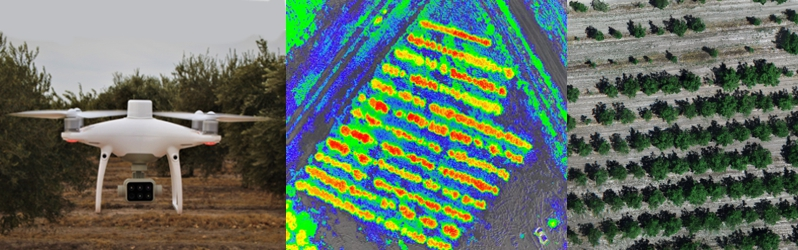
\includegraphics[width=1\textwidth, height=6cm]{./Figures/drones_en_cultivos.jpg}
	\caption{Imágenes tomadas con drones y satélites\protect\footnotemark.}
	\label{fig:drones_en_cultivos}
\end{figure}
\vspace{1cm}

\footnotetext{Imagen tomada de "Monitoreo de cultivos mediante el uso de sensores remotos montados en drones".}

%----------------------------------------------------------------------------------------

\section{Objetivo y alcances}

En esta sección se describen los objetivos del proyecto, los alcances y los aspectos no considerados en el desarrollo del prototipo.

\subsection{Objetivo}

El objetivo del presente trabajo es el desarrollo e implementación de un prototipo que permite contabilizar el rendimiento esperado de un lote de producción de frutos en forma temprana, a través del procesamiento de imágenes.

\subsection{Alcances contemplados}
El alcance establecido para el trabajo incluyó las siguientes tareas:

\begin{itemize}
\item Implementación de un prototipo funcional para la captura automática de imágenes.
\item Desarrollo del firmware que se ejecuta en un sistema operativo de tiempo real.
\item Desarrollo del modelo de detección de objetos.
\item Recolección de imágenes destinadas al proceso de entrenamiento del modelo
\item Establecer como fruto objetivo  de detección el kiwi.
\end{itemize}

%----------------------------------------------------------------------------------------
